\chapter{Introducción}\label{chp:Tema0}

\begin{enumerate}
    \item ¿Qué modelos vamos a estudiar?
    \begin{itemize}
        \item ¿Cómo se ``usan'' los modelos?
        \item ¿Modelos discretos o continuos?
    \end{itemize}
    \item Ejemplos de modelos que vamos a estudiar
    \begin{enumerate}
        \item Dinámica de poblaciones:
        \begin{itemize}
            \item Modelo de Malthus.
            \item Modelo logístico.
            \item Modelo de Leslie.
        \end{itemize}
        \item Modelos aplicados a la economía.
        \begin{itemize}
            \item Interés compuesto.
            \item Ley de la oferta y la demanda (Modelo de la telaraña).
            \item Modelo de la renta de Samelson.
        \end{itemize}
        \item Modelo de Malthus (discreto y continuo). Ejemplo motivador de la asignatura.
        \begin{itemize}
            \item ¿Es el modelo ``bueno''?
            \item Mejoras del modelo $\rightarrow$ Modelo logístico.
        \end{itemize}
    \end{enumerate}
\end{enumerate}

\begin{ejemplo}
    Veamos un ejemplo de interés compuesto. Supongamos que el capital inicial es de 1000€, y el interés anual del 3\%. ¿Cuánto dinero tenemos pasados 5 años?
    \begin{equation*}
        1000\cdot 1.03^5 = 1159.27\text{€}
    \end{equation*}

    Suponiendo que el capital inicial es $c_0$, el número de años viene dado por $n$, y el interés viene dado por $I$, tenemos que:
    \begin{equation*}
        c_n = c_0\left(1+\dfrac{I}{100}\right)^n
    \end{equation*}

    También se puede plantear como una Ley de Recurrencia (también llamada ecuación en diferencias). Es decir:
    \begin{equation*}
        c_{n+1} = c_n\left(1+\dfrac{I}{100}\right)
    \end{equation*}
\end{ejemplo}


\begin{ejemplo}
    Supongamos que estamos estudiando una población de bacterias. Supongamos que la tasa de bacterias que han muerto cada vez que se ve la muestra es de $m=75\%$. Además, supongamos que la tasa de nacimiento es del $f=150\%$. Notando la población de las bacterias por $p_n$, tenemos que:
    \begin{equation*}
        p_{n+1} = p_n + 1.5p_n - 0.75p_n
        = 1.75p_n
    \end{equation*}
    Esto es una ecuación en diferencias, y es un ejemplo del \emph{Modelo de Malthus}. De forma análoga al ejemplo anterior, tenemos que:
    \begin{equation*}
        p_n = 1.75^n\cdot p_0 
    \end{equation*}
    Como $1.75>1$, tenemos que la población crece de forma ilimitada, diverge.
\end{ejemplo}

En estos ejemplos hemos introducido lo que era una ecuación en diferencias. Definámoslo:
\begin{definicion}[Ecuación en diferencias]
    Una ecuación en diferencias (también llamada Ley de Recurrencia) es una relación que se establece entre los términos de una sucesión $\{x_n\}$ de forma que podemos calcular el término $x_{n+1}$ en función de algunos de los anteriores términos mediante una función $f:\bb{R}\times \bb{R}\times \ldots \times \bb{R} \to \bb{R}$ de forma que:
    \begin{equation*}
        x_{n+1} = f(x_n, x_{n-1}, \ldots, x_{n-k})
    \end{equation*}
    A dicha función $f$ se le denomina función asociada a la Ley de Recurrencia.
\end{definicion}
Notemos que, si queremos dar una sucesión que cumpla la ecuación en diferencias dada, será tan simple como dar un término $x_0 \in \bb{R}$ y obligar a que dicha sucesión cumpla la ecuación en diferencias.

Por tanto, resolver una ecuación en diferencias no consistirá en dar una sucesión que cumpla la relación especificada, sino dar una expresión explícita del término $x_n$, para cualquier sucesión que satisfaga la ecuación.

\begin{definicion}[Orden de una ecuación en diferencias]
    Dada una ecuación en diferencias:
    \begin{equation*}
        x_{n+1} = f(x_n, x_{n-1}, \ldots, x_{n-k})
    \end{equation*}
    Diremos que la ecuación es de orden $k\in \bb{N}$.
\end{definicion}
Por tanto, una ecuación de orden 1 será del estilo:
\begin{equation*}
    x_{n+1} = f(x_n)
\end{equation*}

Una ecuación de orden 2 será del estilo:
\begin{equation*}
    x_{n+1} = f(x_n, x_{n-1})
\end{equation*}

\begin{ejemplo}
    Consideremos la ecuación en diferencias dada por $x_{n+2}+x_{n+1}-3=0$. Aunque parezca que se trata de una ecuación de orden 2, en realidad es de orden 1, ya que se puede expresar como $x_{n+1}+x_n -3 = 0$.
\end{ejemplo}

\section{Modelo de Malthus}
Sea $t$ el tiempo, y sea $P(t)$ el tamaño de la población en el tiempo $t$. Sea $f$ la tasa de fertilidad y $m$ la tasa de mortalidad ($0\leq m \leq 1)$.
Tras contar la población pasado un tiempo $\Delta t$, tenemos que:
\begin{align*}
    P(t+\Delta t) &= \text{La que había}
    + \text{Nace} - \text{Muere} =\\
    &= P(t) + \Delta t \cdot f \cdot P(t) - \Delta t \cdot m \cdot P(t) =\\
    &= P(t)\left(\Delta t \cdot (f-m) + 1\right)
\end{align*}

\begin{description}
    \item[Modelo discreto.] Denominando $p_{n+1}=P(t+\Delta t)$, $p_n = P(t)$, tenemos que:
    \begin{equation*}
        p_{n+1} = p_n \cdot \left(\Delta t \cdot (f-m) + 1\right)
    \end{equation*}
    Esta es la ecuación en diferencias.
    Su solución es una \emph{sucesión}.

    También se puede expresar como:
    \begin{equation*}
        p_n = p_0 \left(1+\Delta t(f-m)\right)^n
    \end{equation*}

    Notemos que, debido a que los parámetros se mantienen constantes, será muy común también expresar este modelo como:
    \begin{equation*}
        x_{n+1} = rx_n \qquad r\in \bb{R}^+
    \end{equation*}
    Con $r = \Delta t\cdot (f-m)+1$

    \begin{itemize}
        \item Si $f > m$, tenemos que la población crece.
        \item Si $f < m$, la base de la potencia es menor que 1 y decrece.
    \end{itemize}
    El modelo obliga a la población a reproducirse indefinidamente o a extinguirse, por lo que no es un buen modelo.

    Si nos preguntamos por una solución constante (si nos preguntamos qué pasa si $p_n$ es constante), tendríamos que o bien, $f = m$, o bien $p_n = 0\quad \forall n \in \bb{N}$.

    \item[Modelo continuo.] La tasa de crecimiento es:
    \begin{align*}
        \lim_{\Delta t \to 0} \dfrac{P(t+\Delta t) - P(t)}{\Delta t} &= P'(t) \\
        &= \lim_{\Delta t \to 0} (f-m)P(t) = (f-m)P(t)
    \end{align*}

    Por tanto, tenemos que:
    \begin{equation*}
        P'(t) = (f-m)P(t)
    \end{equation*}
    Esta es la ecuación diferencial.
    Su solución es una \emph{función}.

    Suponiendo que $P(t)$ es siempre positiva o igual a $0$\footnote{No tiene sentido considerar poblaciones con un número negativo de individuos.}:
    \begin{itemize}
        \item Si $f > m$, el producto es positivo y la derivada también $\Rightarrow$ la función crece.
        \item Si $f < m$, el producto es negativo y la derivada también $\Rightarrow$ la función decrece.
    \end{itemize}
\end{description}

De ahora en adelante, apenas consideraremos modelos continuos, y nos centraremos en modelos discretos. Los modelos continuos serán objeto de estudio en la asignatura de Modelos Matemáticos II.

\subsection{Bondad del Modelo de Malthus}
Estudiamos ahora si el Modelo de Malthus es ``bueno''. Algunas desventajas son:
\begin{itemize}
    \item Las tasas de fertilidad y mortalidad constantes no son realistas (al menos para tiempos largos ni para poblaciones grandes de seres vivos).
    \item En el modelo discreto, como hemos visto, la población o crece ilimitadamente o se extingue. No admite comportamientos intermedios.
\end{itemize}
Una ventaja de este es lo sencillo que es de calcular en el caso discreto. En otros modelos, podemos encontrar ecuaciones en diferencias que no seamos capaces de resolver.

\subsection{Solución del Modelo de Malthus}

Veamos en qué consiste resolver una ecuación en diferencias:
\begin{definicion}
    Una sucesión $\{x_n\}$ es una solución de la ecuación $x_{n+1} = f(x_n)$ si satisface la ecuación.
    Es decir, si cada término se obtiene del anterior haciendo su imagen por $f$.
\end{definicion}

La solución del Modelo de Malthus es:
\begin{equation*}
    p_{n} = p_0 \cdot \left(\Delta t \cdot (f-m)+1\right)^n = r^np_0
\end{equation*}


\subsection{Vida Media}

Para el Modelo de Malthus en los casos en los que la población decrece (es decir, en $r\in ]0,1[$), se define la vida media de la siguiente forma:
\begin{definicion}[Vida media en ley de desintegración]
    El tiempo de vida media es el tiempo medio estimado que debe pasar para que una sustancia se desintegre.

    La vida media se define formalmente de la siguiente forma, en el caso de que la sucesión $\sum_{n\geq 0} n(x_{n-1}-x_n)$ converja:
    $$VM := \dfrac{1}{x_0}\sum_{n = 1}^{\infty} n(x_{n-1}-x_n)$$
\end{definicion}

Veamos cómo calcularla de forma concreta en el caso del Modelo de Malthus:
$$x_{n+1} = rx_n\qquad 0 < r < 1$$

Demostremos que se calcula de la siguiente forma:
$$VM := \dfrac{1}{x_0}\sum_{n = 1}^{\infty} n(x_{n-1}-x_n) = \dfrac{1}{1-r}$$

\begin{proof} Partimos de la definición de la vida media:
    \begin{align*}
        VM &= \dfrac{1}{x_0}\sum_{n = 1}^{\infty} n(x_{n-1}-x_n) =\\&
        = \dfrac{1}{x_0} \sum_{n=1}^\infty n(r^{n-1}x_0 - r^n x_0) =\\&
        = \sum_{n=1}^\infty n(r^{n-1}-r^n) = \sum_{n=1}^\infty nr^{n-1} (1-r)=\\&
        = (1-r) \sum_{n=1}^\infty nr^{n-1} \AstIg \dfrac{1-r}{(1-r)^2}
        = \frac{1}{1-r}
    \end{align*}
    donde en $(\ast)$, hemos usado el Lema \ref{lema:SumaInf}, demostrado a continuación.
\end{proof}

\begin{lema}\label{lema:SumaInf}
    $$\sum_{n=1}^\infty n r^{n-1} = \dfrac{1}{(1-r)^2}$$
\end{lema}
\begin{proof}
    Sabemos que:
    \begin{equation*}
        \sum_{i=0}^n r^i = r^0 + r^1 + \dots + r^n = \frac{1-r^{n+1}}{1-r}
    \end{equation*}

    Derivando respeto de $r$, tenemos que:
    \begin{equation*}
        \sum_{i=0}^{n} ir^{i-1} = 1 + 2r + \dots + nr^{n-1} = \frac{-(n+1)r^{n}(1-r) + (1-r^{n+1})}{(1-r)^2}
    \end{equation*}

    Como $|r|<1$, tomando límite con $n\to \infty$, tenemos que:
    \begin{equation*}
        \sum_{n=1}^\infty nr^{n-1} = \sum_{n=0}^\infty nr^{n-1} = \frac{1}{(1-r)^2}
    \end{equation*}
\end{proof}



\section{Modelo Logístico} \label{sec:IntroModeloLogistico}

El presente modelo mejorará el modelo de Malthus. Para concretar los fallos de este último modelo, hemos de incluir las siguientes definiciones (sea $\{p_n\}$ una sucesión de números reales que nos indica el tamaño de población en el $n-$ésimo instante):
\begin{definicion}[Tasa de crecimiento]
    Se define la tasa de crecimiento de una población como:
    \begin{equation*}
        TC :=\dfrac{p_{n+1}}{p_n}
    \end{equation*}

    Nos informa de si la población crece o decrece (mayor o menor que $1$).
\end{definicion}


\begin{definicion}[Tasa neta de crecimiento]
    Se define la tasa neta de crecimiento de una población como:
    \begin{equation*}
        TNC := \dfrac{p_{n+1}-p_n}{p_n} = \frac{p_{n+1}}{p_n}-1 = TC-1
    \end{equation*}

    Nos informa de cuánto crece la población.
\end{definicion}

En el caso del Modelo de Malthus notado de la forma:
\begin{equation*}
    p_{n+1} = r \cdot p_n \qquad 
    \text{con  }  r= 1+\Delta t(f-m)
\end{equation*}

se tendría que:
$$TC = r\qquad TCN = r-1$$

\begin{ejemplo}
    Supongamos un modelo de Malthus dado por:
    $$p_{n+1} = 1.25p_n$$

    Tenemos que:
    \begin{equation*}
        TC = 1.25
        \qquad
        TCN = 1.25 -1 = 0.25
    \end{equation*}
    
    La tasa de crecimiento neto nos dice que la población aumenta en el 25\%.
\end{ejemplo}

El fallo del modelo de Malthus es tener una tasa de crecimiento constante. El modelo logístico resuelve esto. Cambiamos la tasa de crecimiento por una recta de la forma:

$$\dfrac{p_{n+1}}{p_n} = a-b \cdot p_n, \qquad a,b \in \bb{R}^+$$
    
Esto se acerca más a un comportamiento real, ya que conforme la población aumenta, se tiene que:
\begin{itemize}
    \item La tasa de mortalidad $m$ tiende a crecer.
    \item La tasa de fertilidad $f$ tiende a decrecer.
\end{itemize}
Y, conforme la población decrece, se tiene lo contrario, es decir:
\begin{itemize}
    \item La tasa de mortalidad $m$ tiende a decrecer.
    \item La tasa de fertilidad $f$ tiende a crecer.
\end{itemize}

\begin{comment}
Buscamos:
\begin{align*}
    f_n &= \alpha + \beta p_n\\
    m_n &= \gamma + \psi p_n
\end{align*}
Con $\alpha, \beta, \gamma, \psi \in \bb{R}^+$.
\end{comment}

Por tanto, sabiendo la TC, el modelo logístico viene dado por:
\begin{equation*}
    p_{n+1} = p_n (a-b \cdot p_n) \qquad a,b\in \bb{R}^+
\end{equation*}

\begin{observacion}
    ¿Pueden $a,b$ tomar cualquier valor no negativo garantizando que se tenga $p_n \geq 0~~\forall n\in \bb{N}$, suponiendo que $p_0 \geq 0$?\\

    No, veámoslo.
    Para que $p_n\geq 0$, necesitamos que:
    \begin{equation*}
        a-b\cdot p_n \geq 0 \Longleftrightarrow
        a \geq b\cdot p_n
        \Longleftrightarrow
        p_n \leq \frac{a}{b} \qquad \forall n\in \bb{N}
    \end{equation*}

    La función asociada a la ecuación logística es la parábola:
    $$f(x) = x(a-bx)$$
    
    Y, por lo visto anteriormente, necesitamos que la función sea de la siguiente forma: $$f:\left[0, \dfrac{a}{b}\right] \to \left[0, \dfrac{a}{b}\right]$$

    Al valor $\nicefrac{a}{b}$ se le denomina \emph{población tope}.
\end{observacion}

Este modelo no es lineal, como bien podemos ver, ya que su función asociada es una parábola.

%%%%%%%%%%%%%%%%%
% 26 - 2 - 2024 %
%%%%%%%%%%%%%%%%%

\subsection{Solución del Modelo Logístico}

Al contrario de lo que ocurría con Malthus, no podemos buscar una solución a este modelo de forma tan fácil. Veámoslo:
$$x_0 \Rightarrow x_1 = x_0 (a-bx_0) \Rightarrow x_2 = x_1 (a-bx_1) = x_0(a-bx_0)(a-bx_0(a-bx_0))\Rightarrow x_3=...$$
Como vemos, no es fácil encontrar la sucesión de las soluciones. Esto es un caso concreto de un problema de valores iniciales,
que trataremos en la próxima sección.

\section{Soluciones de un modelo.}

Como hemos visto, solucionar una ecuación en diferencias no tiene por qué ser fácil. Se trata de un problema de valores iniciales (PVI).
\begin{definicion}[PVI]
    Un problema de valores iniciales es buscar las soluciones de una ley de recurrencia dado $x_0$ fijado.
    \begin{equation*}
        x_1 = f(x_0) \quad \dots \quad x_{n+1} = f^n (x_0) 
    \end{equation*}
\end{definicion}
Por norma general, resolverlo no es fácil sin el uso de ordenadores, ya que para valores altos de $n$ requiere gran cantidad de cómputos.

\begin{ejemplo} Veamos un ejemplo de PVI particular. Sea la siguiente ecuación en diferencias:
$$x_0=1\qquad x_{n+1}=\log(x_n)$$

En este caso, se resuelve de forma sencilla, ya que $x_1=0$ y ya no se puede continuar, ya que no pertenece al dominio de definición del logaritmo.

\begin{observacion}
    Veamos si podemos encontrar $I\subset \bb{R}$ tal que si tomamos $x_0\in I$ la sucesión dada por la Ley de Recurrencia $x_{n+1}=\log(x_n)$ tenga infinitos términos.
\end{observacion}
\end{ejemplo}

%%%%%%%%%%%%%%%%%
% 27 - 2 - 2024 %
%%%%%%%%%%%%%%%%%

La ecuación en diferencias siempre viene asociada a una funciónf $f$ dada por:
$$f:I \rightarrow \bb{R}\qquad x_{n+1} = f(x_n)$$
Basta que $f(I) \subseteq I$ para poder sacar una sucesión que resuelva el PVI.

\begin{definicion}[Órbita o trayectoria]
    Se define la órbita o trayectoria de la solución que empieza en $x_0$ como:
    $$ \{ x_0, f(x_0), (f\circ f)(x_0), \ldots, f^{n}(x_0), \ldots \}$$
    Esta es la sucesión de todos los términos de la solución de un modelo.
\end{definicion}
\begin{definicion}[Retrato de fases]
    El retrato de fases es la representación gráfica de la órbita.
\end{definicion}
\begin{ejemplo} Resolver el modelo de Malthus dado por:
    $$x_{n+1} = 2x_n$$
    Dado $x_0$, la solución tiene término general $x_n = 2^n x_0$.\newline
    $$\text{órbita}_{x_0} = \{ x_0, 2x_0, 2^2 x_0, \ldots, 2^n x_0, \ldots \} $$
    Su retrato de fases sería el siguiente: 
    \begin{figure}[H]
        \centering
        \begin{tikzpicture}
          % Dibujar la recta real
          \draw (-1,0) -- (10,0);
          
          % Dibujar las potencias de 2
          \draw (0,0.15) -- (0,-0.15) node[below] {$0$};
          \draw (1,0.15) -- (1,-0.15) node[below] {$x_0$};
          \draw (2,0.15) -- (2,-0.15) node[below] {$x_1$};
          \draw (4,0.15) -- (4,-0.15) node[below] {$x_2$};
          \draw (8,0.15) -- (8,-0.15) node[below] {$x_3$};

          \draw[dashed, ultra thick, -stealth] (1,0) -- (1.1,0);
          \draw[dashed, ultra thick, -stealth] (2,0) -- (2.1,0);
          \draw[dashed, ultra thick, -stealth] (4,0) -- (4.1,0);
          \draw[dashed, ultra thick, -stealth] (8,0) -- (8.1,0);
        
          \begin{comment}
          \draw[dashed, -stealth] (1,0) arc (180:0:0.5);
          \draw[dashed, -stealth] (2,0) arc (180:0:1);
          \draw[dashed, -stealth] (4,0) arc (180:0:2);
          \draw[dashed] (8,0) arc (180:120:4);
          \end{comment}
        \end{tikzpicture}
        \caption{Retrato de fases del modelo de Malthus dado por $x_{n+1}=2x_n$.}
    \end{figure}
    La función $f$ asociada sería:
    \Func{f}{\bb{R}}{\bb{R}}{x}{2x}
    
    La ecuación tiene sentido para cualquier dato de $\bb{R}$. Sin embargo, si tratamos el modelo de Malthus en poblaciones (por ejemplo), no tiene sentido considerar todo~$\bb{R}$.
\end{ejemplo}

\begin{definicion}[Soluciones constantes]
    Una solución constante, también llamado punto de equilibrio, es una órbita que es una sucesión constante 
    $ x_c = \{x_n\}_{n\geq 0}$ que cumplen la ecuación $x_{n+1} = f(x_n)$ y que tienen todos sus términos iguales:
    $$x_c = \{ c, c, \ldots, c, \ldots \} $$
    Es decir; se trata de encontrar $c \in I$ tal que $c = f(c)$. Determinamos entonces las soluciones constantes encontrando los puntos fijos de $f$.
\end{definicion}
\begin{ejemplo}
    \noindent
    Si el modelo fuera $x_{n+1} = 0 \cdot x_n$, la órbita sería:
    $$\{0, 0, \ldots, 0, \ldots \}$$
    Se trata de una solución constante, con retrato de fases:
    \begin{figure}[H]
        \centering
        \begin{tikzpicture}
          % Dibujar la recta real
          \draw (-2,0) -- (2,0);
          
          % Dibujar las potencias de 2
          \draw (0,0.15) -- (0,-0.15) node[below] {$0$};
          \fill[black] (0,0) circle (2pt);

          %\draw[dashed, ultra thick, -stealth] (1,0) -- (1.1,0);
          
        \end{tikzpicture}
        \caption{Retrato de fases del modelo de Malthus dado por $x_{n+1}=0\cdot x_n$.}
    \end{figure}
\end{ejemplo}


Centrémonos ahora en hallar las soluciones constantes de los modelos vistos hasta el momento. Trabajemos con el modelo de \textbf{Malthus} dado por:
$$x_{n+1} = r \cdot x_n$$
Las soluciones constantes son:
\begin{itemize}
    \item \ul{Si $r \neq 1$}:
    Entonces $x_c = 0$, $c = 0$.
    \item \ul{Si $r=1$}:
    $x_{x_0} = \{ x_0, x_0, \ldots, x_0, \ldots \}$, con $x_0 \in \bb{R}$.
\end{itemize}

Para el modelo \textbf{logístico} dado por: $$p_{n+1} = p_n(a-b\cdot p_n)\qquad 0 \leq p_0 \leq \dfrac{a}{b}$$

Las soluciones constantes son:
$$x_0 = \{0, 0, \ldots, \}$$
$$x_{\frac{a-1}{b}} = \left\{ \dfrac{a-1}{b}, \dfrac{a-1}{b}, \ldots \right\}$$

Veamos cómo las hemos obtenido. La $f$ asociada es: $f(x) = x(a-bx)$, por lo que los puntos fijos son las soluciones de la ecuación $c=c(a-bc)$.
\begin{itemize}
    \item $c = 0$
    \item $c = \dfrac{a-1}{b}$
\end{itemize}

\begin{definicion}[Ciclos]
Un $n$-ciclo es una solución de la ecuación que cumple que $x_n = x_0$, es decir:
$$f^n(x_0) = x_0$$
Por tanto, los puntos fijos de $f^n$ son los $n-$ciclos. La órbita de un $n$-ciclo es de la forma:
$$\{x_0, x_1, x_2, \ldots, x_{n-1}, x_0, x_1, x_2, \ldots, x_{n-1}, x_0, x_1, x_2, \ldots \}$$

Para que los ciclos sean no triviales, sus elementos no deben ser puntos fijos de $f^m$, con $m<n$.
\end{definicion}

\begin{ejemplo}
    Sea el modelo dado por:
    $$x_{n+1} = -x_n$$
    La $f$ asociada es $f:\bb{R} \rightarrow \bb{R}$ dada por: $f(x) = -x$. Su órbita es:
    $$\text{Órbita}_{x_0} = \{x_0, -x_0, x_0, -x_0, \ldots \}$$
    Se trata de un $2$-ciclo. El retrato de fases sería el siguiente:
    \begin{figure}[H]
        \centering
        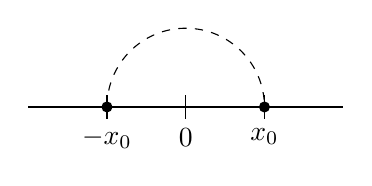
\begin{tikzpicture}
          % Dibujar la recta real
          \draw (-2,0) -- (2,0);
          
          % Dibujar las potencias de 2
          \draw (-1,0.15) -- (-1,-0.15) node[below] {$-x_0$};
          \draw (0,0.15) -- (0,-0.15) node[below] {$0$};
          \draw (1,0.15) -- (1,-0.15) node[below] {$x_0$};
          \fill[black] (-1,0) circle (2pt);
          \fill[black] (1,0) circle (2pt);
          
          \draw[dashed] (-1,0) arc (180:0:1);
          
        \end{tikzpicture}
        \caption{Retrato de fases del modelo de Malthus dado por $x_{n+1}=-x_n$.}
    \end{figure}
\end{ejemplo}

Veamos ahora qué ocurre en el caso de que no se pueda calcular de forma explícita la solución constante del modelo.
\begin{figure}[H]
    \centering
    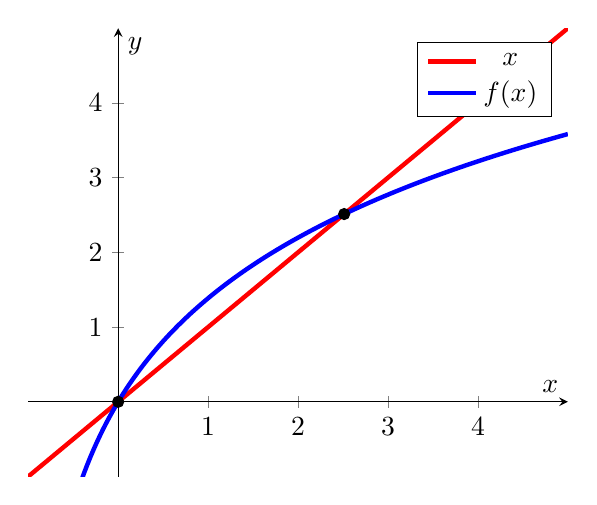
\begin{tikzpicture}
    \begin{axis}[
        axis lines=middle,
        xlabel={$x$},
        ylabel={$y$},
        xmin=-1, xmax=5,
        ymin=-1, ymax=5,
        xtick={1,2,3,4},
        ytick={1,2,3,4},
        yticklabels={$1$,$2$,$3$,$4$},
        xticklabels={$1$,$2$,$3$,$4$},
        domain=-2:5,
        samples=200,
        legend pos=north east, % Cambia la posición de la leyenda
        ]
        \addplot[red, ultra thick] {x} node[right] {$x$};
        \addplot[blue, ultra thick] {2*ln(1+x)} node[right] {$f(x)$};
        \legend{$x$, $f(x)$};

        % Marcando los puntos de intersección
        \addplot[mark=*] coordinates {(0,0)};
        \addplot[mark=*] coordinates {(2.512862417), (2.512862417)};
    \end{axis}
    \end{tikzpicture}
\end{figure}
Como bien podemos observar, las soluciones constantes serán los puntos de corte entre las gráficas $y=x$ y la función asociada al modelo $f$. El trabajo con gráficas será muy común en esta asignatura para entender resultados intuitivos.

\begin{comment}
\begin{ejercicio*}
    Estudiar el modelo dado por:
    $$x_{n+1} = i \cdot x_n$$
    donde $i$ es la unidad imaginaria.

\end{ejercicio*}
\begin{ejercicio*}
    Estudiar el modelo dado por:
    $$x_{n+1} = r\cdot x_n \qquad r \in \bb{C}~|r| =1$$
\end{ejercicio*}
\end{comment}


\begin{comment}
\section{Estabilidad}
En esta sección, veremos cómo sabemos qué hace el modelo si no conocemos el término general (es decir, una fórmula explícita).


\begin{definicion}[Estabilidad]
    Decimos que $x = c$ es estable si las soluciones que empiezan cerca de $x = c$, se quedan cerca de $x = c$. Es decir:
    $$\forall \varepsilon > 0 \qquad\exists \delta>0, \text{ Si } x_0 \in \bb{R},~ |x_0 - c| < \delta \Longrightarrow |x_n -c| < \varepsilon\qquad \forall n\in \bb{N}$$

    De forma evidente, se tiene que las soluciones constantes son estables.
\end{definicion}

\begin{definicion}[Estabilidad asintótica]
    Decimos que $x = c$ es asintóticamente estable si, además de ser estable, se tiene que $\lim\limits_{n \to \infty} x_n = c$ si $x_0$ está cerca de $c$.
\end{definicion}
\begin{ejemplo}
    \noindent
    Por ejemplo, consideramos los modelos de Malthus dados por:
    $$x_{n+1} = 0.9 \cdot x_n \qquad x_{n+1} = 1.2 \cdot x_n \qquad x_{n+1} = -x_n$$
    Las soluciones constantes de todas son $c = 0$.
    
    En la última, cabe destacar que
    $x_0 = 0$ es estable (es una solución cosntante) pero no asintóticamente estable, ya que si $x_0\neq 0$ entonces
    $\lim\limits_{n \to \infty} x_n \neq 0$.
\end{ejemplo}
\end{comment}

\begin{comment}
\section{Linealización}
En el caso no modelos no lineales, ¿cómo miramos la estabilidad de las soluciones constantes? La idea es linealizar el modelo mediante la serie de Taylor. Dada nuestra ecuación:
$$x_{n+1} = f(x_n)$$
Y supongamos que $f(c) = c \Rightarrow x_c = \{ c,c, \ldots \}$ es una solución constante.

El desarrollo de Taylor de orden 1 centrado en $c$ es:
$$f(x) = f(c) + f'(\gamma)(x-c)
\qquad \gamma \text{ entre $c$ y $x$}.$$

Tenemos entonces que:
$$f(x) = f(c) + f'(\gamma)(x-c) \Longrightarrow f(x) = c + f'(\gamma)(x-c)$$

Suponemos que $x_0$ está ``cerca'' de $c$.
$$x_0 \Longrightarrow x_1 = f(x_0) = c + f'(\gamma)(x_0-c) \Longleftrightarrow |x_1-c| = |f'(\gamma)||x_0-c|$$
con $\gamma$ entre $c$ y $x$.
Por esa última igualdad, tenemos el siguiente resultado:
\begin{itemize}
    \item \ul{Si $|f'(c)|<1$:}
    Tenemos que $\alpha_c = \{c, c, \ldots\}$ es asintóticamente estable.
    \item \ul{Si $|f'(c)|>1$:}
    Tenemos que: $\alpha_c = \{c, c, \ldots\}$ es inestable.
    \item \ul{Si $|f'(c)| =1$:}
    No aporta información.
\end{itemize}
Este resultado lo veremos próximamente en teoría de forma más profunda.

\end{comment}